\documentclass[tikz]{standalone}
\renewcommand*\familydefault{\sfdefault}
\usetikzlibrary{calc,trees,positioning,arrows,chains,shapes.geometric,%
    decorations.pathreplacing,decorations.pathmorphing,shapes,%
    matrix,shapes.symbols,fit}

\pgfdeclarelayer{back}
\pgfsetlayers{back,main}


\makeatletter
\tikzset{
  fitting node/.style={
    inner sep=0pt,
    fill=none,
    draw=none,
    reset transform,
    fit={(\pgf@pathminx,\pgf@pathminy) (\pgf@pathmaxx,\pgf@pathmaxy)}
  },
  reset transform/.code={\pgftransformreset}% ,
  % node/.append style={text color=white, color=white}
}
\makeatother


\begin{document}
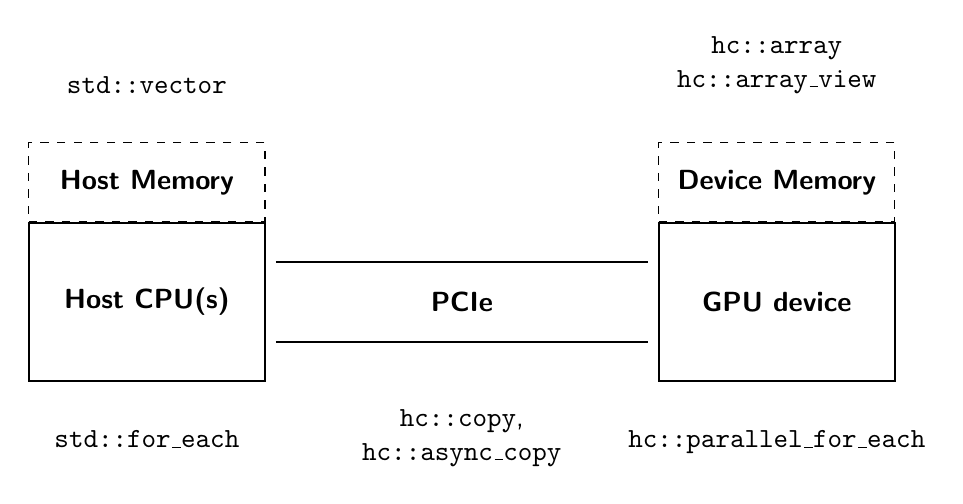
\begin{tikzpicture}[% every node/.style={color=white}
  ]

  \node [draw,thick,rectangle, minimum width=3cm, minimum height=2cm] at(0,0) (host) {\bfseries{}Host CPU(s)};
  \node [draw,dashed,rectangle, minimum width=3cm, minimum height=1cm, anchor=south] at (host.north)(host_memory) {\bfseries{}Host Memory};

  \node [draw,thick,rectangle, minimum width=3cm, minimum height=2cm] at($(host)+(8,0)$) (device) {\bfseries{}GPU device};
  \node [draw,dashed,rectangle, minimum width=3cm, minimum height=1cm, anchor=south] at(device.north) (device_memory) {\bfseries{}Device Memory};

  \node at($(host.east)!.5!(device.west)$) (pcie) {\bfseries{}PCIe};

  \node at($(host.east)!.5!(host.north east)$) (pcie_topleft) {};
  \node at($(host.east)!.5!(host.south east)$) (pcie_botleft) {};

  \node at($(device.west)!.5!(device.north west)$) (pcie_topright) {};
  \node at($(device.west)!.5!(device.south west)$) (pcie_botright) {};

  \draw [thick% ,color=white
  ] (pcie_topleft) -- (pcie_topright);
  \draw [thick% ,color=white
  ] (pcie_botleft) -- (pcie_botright);


  %decripe hc API

  \node [above=5mm of host_memory] (stdvec) {\texttt{std::vector}};
  \node [above=5mm of device_memory,text width=3cm, align=center] (hcarr) {\texttt{hc::array} \texttt{hc::array\_view}};
  
  \node [below=of pcie, text width=4cm, align=center] (stdvec) {\texttt{hc::copy}, \texttt{hc::async\_copy}};

  \node [below=5mm of device, align=center] (stdvec) {\texttt{hc::parallel\_for\_each}};

  \node [below=5mm of host, align=center] (stdvec) {\texttt{std::for\_each}};

\end{tikzpicture}
\end{document}
